\chapter{Généralités sur les réseaux de capteurs sans fil}
\section{Introduction}
        Le progrès technologique qu'a connu le domaine des réseaux sans fil et de la micro-électronique ont permis le développement de micro-composants intégrant des dispositifs de captage, de calcul et de communication sans fil, dans un même circuit, de petite dimension et à cout réduit nommé capteur sans fil pouvant détecter, mesurer, recueillir et partager de l'information sur son environnement.\\
         Ces nouveaux composants  ont donné naissance à un tout nouveau type de réseaux, il s'agit des réseaux de capteurs sans fil (RCSFs), il s'agit d'un travail collaboratif entre un nombre important de capteurs sans fil déployés sur une surface géographique donné dans le but de collecter des données relatives à un phénomène à observer.  \\
         Ces réseaux initialement dédiés au domaine militaire, ont actuellement envahi presque tous les secteurs,  de l'industrie, à la médecine, en passant par le domaine des transports et l'environnement.
        
        %Pour déclarer une nouvelle abréviation
        \nomenclature{RCSF}{Réseau de capteurs sans fil}
        
     A travers ce chapitre, nous allons commencer par une présentation des réseaux sans fil, puis une description et une architecture d'un capteur sans fil seront présentés pour passer aux réseaux de capteurs sans fil à travers  une description globale de ces réseaux, leurs architectures, leurs contraintes de conception, ainsi leurs domaines d'utilisation.
        
\section{Les réseaux sans fil} 
 Les réseaux sans fil se sont de plus en plus répandu au fil des années, les liaisons filaires permettant l'accès au réseau se font désormais rare, cela est due à la flexibilité offerte par le sans fil et la forte apparition des  unités de calcul mobiles (smartphones, tablettes, laptops, PDA...), plusieurs normes et  technologies de transmission sans fil se sont développées (WiFi, BlueThooth, ZigBee...) selon le domaine d'utilisation et la portée de la transmission.\\
 Les réseaux sans fil peuvent être classé selon plusieurs critères, nous nous intéresserons à leur classement   selon la présence ou l'absence d'une infrastructure administrant le réseau.
\begin{itemize}
\item \textbf{Les réseaux avec infrastructure: }Dans ce type de réseaux, une infrastructure est mise en place pour l'administration du réseau généralement un point d'accès, les périphériques au sein ce réseau ne peuvent pas communiquer directement, les communications doivent passer obligatoirement par le point d'accès. 

\item \textbf{Les réseaux sans infrastructure: }Les réseaux sans infrastructure appelés aussi réseaux Ad-Hoc, ne comportent pas d'infrastructure centralisé administrant le réseau, les nœuds voisins communiquent directement entre eux, les nœuds s'auto-organisent afin d'effectuer les processus de routage et d'acheminement de données, cette décentralisation offerte par ces réseaux ouvre la voix à plusieurs types d'applications, les réseaux de capteurs sans fil dont nous allons présenter est un type particulier de ces réseaux.
\end{itemize}
\section{Les capteurs sans fil}
	\subsection{Qu'est qu'un capteur?}
	Un capteur sans fil est un objet physique de petite taille peu couteux, sa fonctionnalité principale est de détecter et mesurer des phénomènes physiques l'environnant, ces données récupérées seront par la suite converties en données numériques pour une exploitation future. Un capteur est alimenté généralement par des batteries ne pouvant ni se rechargé ni se remplacé dans la majorité des cas, ce qui rend la consommation énergétique un des défis majeurs pour la conception et le déploiement des réseaux de capteurs sans fil.\\ La figure \ref{capteur} ci-dessous illustre un modèle réel de capteur sans fil:
	\begin{figure}[h]
	\begin{center}
	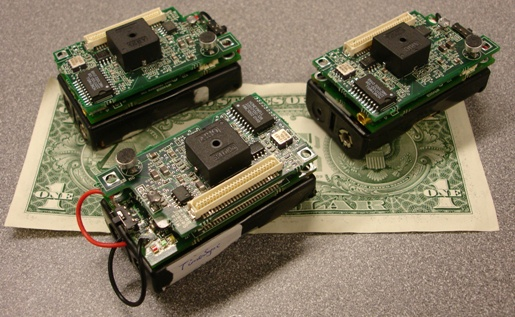
\includegraphics[scale=0.5]{Chapitre1/capteur.jpg}
	\caption{\label{capteur}Exemple d'un capteur sans fil}
	\end{center}
	\end{figure}
	
	
	
	
	\subsection{Architecture d'un capteur sans fil}
	Afin d'accomplir ses fonctions principales un capteur est généralement composé de quatre unités principales à savoir une unité de capture, de traitement, de communication et une unité d'alimentation.
	\begin{itemize}
		\item \textbf{Unité de capture}: L'unité qui caractérise le capteur selon son domaine d'application, elle permet de récupérer des grandeurs physiques à partir de l'environnement (température, pression, son...) à travers des capteurs, ces grandeurs seront par la suite converties en grandeurs numériques pour être exploitées par l'unité de traitement, cette unité est composé donc de deux sous unités, la première effectue les opérations de captage, la deuxième quant à elle, elle s'occupe de la conversion des données analogiques acquises en données numériques. \\

		
		\item \textbf{Unité de traitement:} Il s'agit de l'unité intermédiaire entre l'unité de capture et l'unité de communication, elle est dotée d'un processeur et d'un système d'exploitation spécifique, son rôle est de récupérer les données acquises par l'unité de capture, d'effectuer quelques traitements sur les données pour les transmettre par la suite vers l'unité de communication. \\
		
		
		\item \textbf{Unité de communication:}L'unité responsable de communiquer les données acquises par le capteur vers l'extérieur (capteurs avoisinants), à travers un support de communication radio. \\ 

		
		\item \textbf{Unité d'alimentation:}L'unité en charge de fournir l'énergie nécessaire au fonctionnement des trois autres unités, il s'agit dans la majorité des cas de batteries ne pouvant être ni rechargés ni remplacés vu l'environnement hostile de déploiement des capteurs.
	\end{itemize}
	
	
	
	
	\begin{figure}[h]
		\begin{center}
			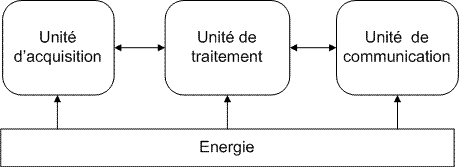
\includegraphics[scale=0.7]{Chapitre1/architecture_capteur.png}
		\end{center}
		\caption{Architecture de base d'un capteur sans fil}
	\end{figure}
	
	Il est à noter qu'en plus de ces unités de base, les capteurs peuvent être dotés d'autres unités additionnels selon leurs domaines d'applications, (eg: unités permettant la mobilité des capteurs, unités permettant la localisation des capteurs...etc).
	
	\subsection{Les systèmes d'exploitation des capteurs sans fil}
 Les systèmes d'exploitation jouent le rôle de gestionnaires de ressources dans un système informatique, une gestion efficace et équitable est primordiale. Or dans le cas des capteurs sans fil les ressources sont extrêmement limitées ce qui impose de nouveaux défis de conception des systèmes d'exploitation destinés aux capteurs sans fil par rapport aux systèmes d'exploitation traditionnels.\\
 Plusieurs facteurs devraient être pris en considération lors de la conception d'un système d'exploitation destiné au capteurs sans fil à savoir:
 \begin{itemize}
 \item \textbf{Taille réduite du système: }La mémoire limitée des capteurs sans fil (à l'ordre de quelques kilo bits), impose une taille réduite du système d'exploitation. 
 
 \item \textbf{Gestion de l'énergie: }Le système d'exploitation devraient fournir des mécanismes de gestion et d'économie d'énergie, par exemple éteindre certains périphériques lorsque le capteur est au repos et les rallumer à la suite d'interception d'événements.
 
 \item \textbf{L'ordonnancement des processus: }Les ordonnanceurs dans les systèmes d'exploitation classique avaient pour objectifs de réduire la latence et de maximiser l'utilisation des ressources, dans le cas des RCSFs l'algorithme d'ordonnancement devraient satisfaire les exigences de l'application tout en minimisant l'utilisation de la mémoire et de l'énergie. 
 
 \item \textbf{Protection et gestion de la mémoire: }Dans un système d'exploitation classique chaque processus dispose de son propre espace d'adressage, ce mécanisme ne pouvant être appliqué pour les capteurs sans fil vu la taille réduite de la mémoire disponible, un mécanisme de partage de la mémoire devrait être mise en place.
 
 \item \textbf{Support de protocoles de communication: }Un RCSF étant un système distribué de capteurs sans fil, le système d'exploitation doit offrir une interface de programmation (API) permettant aux applications de communiquer tout en prenant en considération l'hétérogénéité des nœuds composant le réseau. 

 \end{itemize}
 
 Plusieurs systèmes d'exploitation destinés aux capteurs sans fil se sont développés au fil du temps, parmi les systèmes les plus populaires, on distingue: TinyOS, Contiki, MANTIS, LiteOS.




		 \newpage

\section{Les réseaux de capteurs sans fil}
\subsection{Définition}
Un réseau de capteurs sans fil, est un ensemble de capteurs  sans fil -appelés nœuds- spatialement distribué sur une surface nommée \emph{champ de captage}, ces nœuds sont capables d'interagir avec leur environnement en détectant et mesurant des paramètres physiques de ce dernier(température, pression, bruit, mouvement, lumière...), ces paramètres sont échangées entre les nœuds à travers des ondes radio jusqu'à ce qu'ils atteignent une station de base externe au champ de captage, cette station appelée station puits (ou point de récolte) (\emph{sink} en anglais) peut utiliser les données récoltées localement ou elle les transmet à son tour  à un utilisateur final à  travers le réseau(réseau local, par satellite, via internet...). L'utilisateur peut aussi envoyer des requêtes au réseau à travers cette station de base qui considérée comme une passerelle.
La figure ci-dessous représente un exemple d'architecture d'un réseau de capteurs sans fil:
\begin{figure}[h]
\begin{center}
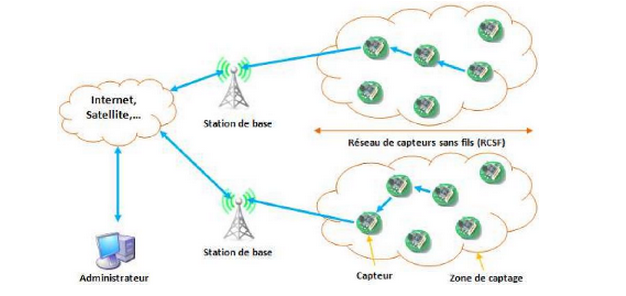
\includegraphics[scale=1]{Chapitre1/wsn_archi.png}
\caption{Architecture d'un réseau de capteurs sans fil (RCSFs)}
\end{center}
\end{figure}


\subsection{Contraintes de conception des RCSFs }
Les réseaux de capteurs sans fil (RCSFs), sont omniprésents dans de nombreux secteurs, et dans de nombreuses applications, cette diversification d'application est due  à une certaine flexibilité offerte par ces réseaux, à titre d'exemple la diversité des capteurs existants, la mobilité des nœuds, la possibilité d'utilisation de ces réseaux dans des milieux hostiles...etc, cette diversification à pour conséquences des défis de conception majeurs afin d'adapter chaque réseau à son domaine d'application, car les exigences diffèrent selon l'application.
Parmi ces contraintes on peut citer:

\begin{itemize}
\item \textbf{Durée de vie du réseau}: Elle diffère selon les domaines d'applications, elle peut varier de quelques jours à plusieurs années, elle correspond à la durée entre la mise en place du réseau et l'épuisement de l'énergie des capteurs su réseau.\\

\item \textbf{Limitation des ressources}: Les capteurs disposent de ressources limitées en terme de bande passante, puissance de calcul, mémoire...etc, cela afin de garantir une taille réduite et un prix abordable au capteur. La conception d'un RCSF doit prendre en considération ces limitations.\\

\item \textbf{Topologie dynamique}: La topologie du réseau peut varier à travers le temps, cela est due à plusieurs facteurs comme: la possibilité de mobilité des nœuds dans certaines applications, l'épuisement de l'énergie d'un nœud du réseau, la défaillance d'un nœud...etc, le réseau devrait s'adapter automatiquement à ces changements.\\

\item \textbf{Le temps de réponse}: Dans certaines applications, le temps de réponse est un des facteurs critiques de conception du réseau, (eg: dans le cas des stations nucléaires), dans ce genre d'applications il faudrait mettre l'accent sur le temps, même s'il peut affecter la durée de vie du réseau, il faudrait faire un compromis lors de la conception.\\

\item \textbf{La scalabilité du réseau}: La scalabilité  du réseau (adaptation à l'échelle), est un des critères clé de conception des RCSFs, le réseau devrait s'adapter à l'ajout des nœuds au fil du temps.\\


 

\end{itemize}



\subsection{Domaines d'application des RCSFs}
Les réseaux de capteurs sans fil initialement dédiés au domaine militaire ont envahi ces dernières années la majorité des secteurs, cela est due au développement qu'a connu ce type de réseau en terme matériel et logiciel, la miniaturisation et la réduction des coûts des capteurs, ainsi l'impact que peuvent apporter ces derniers  dans les différents secteurs. Parmi les domaines où ces réseaux ont eu un fort impact on retrouve le domaine médical, l'industrie, l'environnement, l'architecture (Maisons et structures intelligentes).  
\begin{itemize}
		\item \textbf{Applications militaires}: Les RCSFs étaient initialement dédiés au domaine militaire, avant de s'élargir vers les autre secteurs, ils ont la capacité d'être déployés dans des environnements hostiles (champ de bataille par exemple) ou l'intervention humaine est quasiment impossible, il permettent de collecter pas mal d'information, des informations sur les troupes (positionnement, armement ...) et des informations sur les ennemis(lieux de présence, nombre,  ...), ils peuvent aussi être utilisés dans le cas de détection des attaques chimiques et biologiques.\\  

		\item \textbf{Applications médicales}: Les réseaux de capteurs sans fil peuvent être utilisé pour récupérer 
		des données physiologiques des patients (pression artérielle, fréquence cardiaque...etc), ces données permettent une surveillance à distance des patients et une meilleure réactivité en cas d'urgence, les capteurs sans fil peuvent aussi être administrés comme étant des gelules, permettant de transmettre des images en temps réel de l'intérieur du corps sans recourir à la chirurgie, .\\
		
		\item \textbf{Applications environnementales}: Les RCSFs ont connu un progrès remarquable dans les applications environnementales, ils permettent la détection des incendies, des inondations, des fuites de produits dangereux (gaz, produits chimiques, éléments radio-actifs...). Ils peuvent aussi être utilisé pour le suivi des plantes et des animaux. \\
		
		\item \textbf{Applications domestiques}: Les RCSFs se sont introduits même dans les habitations, les capteurs sont intégrés dans pas mal d'appareils électroménagers (aspirateurs, réfrigérateur, machine à laver ...), ils permettent  la détection des problèmes, l'interaction avec les appareils à distance et d'une manière confortable par les utilisateurs finaux. Ils sont aussi utilisés pour réguler la température au sein de l'habitation d'une manière automatique tout en réduisant la consommation énergétique.\\
		
		\item \textbf{Applications routières}: Les RCSFs peuvent apporter une aide considérable dans la gestion routière, ils permettent en conséquence un gain de temps considérable pour les automobilistes ainsi une réduction de la consommation énergétique et du taux de pollution, ils sont utilisés pour la gestion des carrefours (gestion intelligentes des feux tricolores selon la présence et le flux des véhicules), la gestion intelligente des parkings (détection des emplacements vides et de la surcharge de la structure automatiquement) et pas mal d'autres applications intelligentes facilitant la vie des automobilistes.\\
				
\end{itemize}

\subsection{La communication dans les RCSFs}
Un réseau de capteurs sans fil étant composé de plusieurs nœuds déployés dans un environnement supervisé, la puissance de ces réseaux figure dans la possibilité de coopération entre ces nœuds afin de transmettre des informations sur l'environnement supervisé, pour assurer cette coopération des mécanismes de communication devraient être mise en place pour assurer une communication efficace répondant aux exigences des capteurs sans fil (en termes de limitation de ressources et d'énergie).\\
A cet effet, une pile protocolaire à été mise en place semblable à celle du modèle OSI afin de faciliter et standardiser la communication au sein des RCSFs, la pile protocolaire mise en place pour les RCSFs comprend 5 couches (La couche application, transport, réseau, liaison de données, et la couche physique) et 3 plans de gestion (Plan de gestion de l'énergie, plan de gestion de mobilité et un plan de gestion des tâches) résumés dans la figure ci-dessous:

\begin{figure}[h]
\begin{center}
	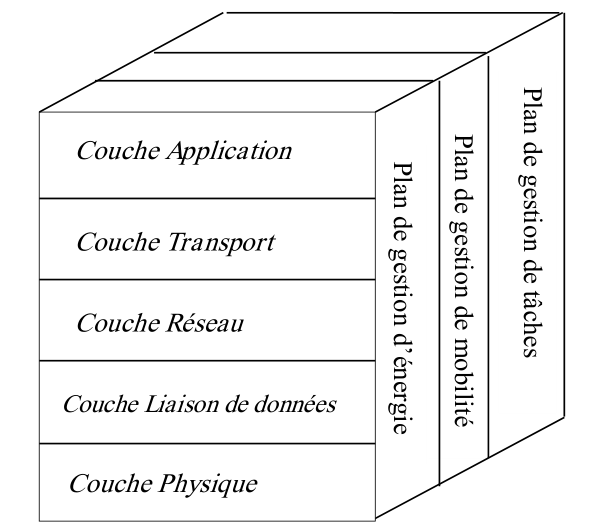
\includegraphics[scale=0.6]{Chapitre1/pile.png}
	\caption{La pile protocolaire dans les réseaux de capteurs sans fil}
\end{center}
\end{figure}

\subsubsection{Description des couches de la pile protocolaire}
\begin{itemize}
\item \textbf{La couche application:}Elle représente l'interface avec les applications, il s'agit de la couche la plus proche des utilisateurs finaux, de nombreuses applications peuvent être mise en place au niveau de cette couche à titre d'exemple SMP(Sensor Management Protocol), TADAP(Task Assignement and Data Advertissement Protocol), SQDDP(Sensor Query and Data Dissemination protocol).\\
  La couche application a pour mission principale le traitement de l'information détectée (ou mesurée), son encodage, sa mise en forme et la manière de stockage et de transfert de cette information. Elle a aussi pour rôle de vérifier la disponibilité des ressources pour répondre aux exigences du réseau en communiquant avec les couches sous-jacentes.\\
  
  \item \textbf{La couche transport:}Elle est  responsable de l'acheminement des données de manière transparente et fiable (Dans certaines applications la fiabilité n'est pas primordiale), de la segmentation des données venant de la couche application, réordonnancent des segments provenant de la couche réseau, ainsi le contrôle de flux et la gestion des erreurs. 
  
  
  \item \textbf{La couche réseau:} Elle est responsables du routage des données, en établissant les chemins optimaux entre les nœuds et les stations puits, dans les RCSFs l'accent est mis sur la consommation énergétique lors de l'établissement des routes.\\
  Le routage dans les RCSFs diffère de celui des réseaux AD-HOC cela est due aux caractéristiques particulières des RCSFs à savoir:
  \begin{itemize}
  \item Impossibilité d'établir un schéma d'adressage global.
  \item	Limitation de l'énergie et des ressources des capteurs sans fil.
 \item Redondance des données produite par des capteurs adjacents couvrant partiellement la même région géographique.
 \item Les routes devraient relier des sources multiples (capteurs sans fil) vers une seule destination (station de base).\\
  \end{itemize}
  
  \item \textbf{La couche liaison de données:} Elle spécifie la façon d'expédition des données entre deux nœuds, dont la distance entre eux est d'un seul saut, elle est aussi responsable du multiplexage des données, du contrôle d'erreurs et du contrôle de l'accès au média.   \\
  
  \item \textbf{La couche physique:}  Elle est responsable des caractéristiques physiques (matérielles) de la communication, comme la génération des ondes et la détection des signaux, elle responsable de l'acheminement et de la réception des données au niveau bit.   \\ 
\end{itemize}


\subsubsection{Les plans de gestion:}
En plus des 5 couches vus précédemment, la communication dans les RCSFs se fait à base de 3 plans de gestion, assurant une communication efficace, une meilleure coordination des taches tout en minimisant la consommation énergétique.

\begin{itemize}
 \item \textbf{Plan de gestion de l'énergie:}A pour rôle principal la gestion efficace de la consommation énergétique au sein du réseau lors des phases de détection, de traitement et de la communication en utilisant divers mécanismes, comme l'extinction du récepteur des messages lors de la réception d'un message pour éviter la réception et le traitement des messages dupliqués, ou bien encore signaler le faible niveau d'énergie atteint par nœud afin que ce dernier ne participe plus au processus de routage.\\
 
 \item \textbf{Plan de gestion de la mobilité:}A pour rôle la détection, le suivi et l'enregistrement des mouvements des nœuds voisins  pour garder une image récente du voisinage d'un nœud à tout moment, cette image sert pour les plan de gestion des tâches et d'énergie en effectuant un équilibrage de tâches et de consommation énergétique entre les nœuds (Deux nœuds couvrant la même région géographique ne doivent pas travailler en même temps).  \\
 
 \item \textbf{Plan de gestion des tâches:}A pour rôle l'équilibrage de l'affectation des tâches entre les nœuds du réseau, ce qui garantit une meilleure consommation énergétique donc augmentation de la durée de vie du réseau.

\end{itemize}	
   
 
 